% (find-LATEX "2021-2-C2-intro.tex")
% (defun c () (interactive) (find-LATEXsh "lualatex -record 2021-2-C2-intro.tex" :end))
% (defun C () (interactive) (find-LATEXsh "lualatex 2021-2-C2-intro.tex" "Success!!!"))
% (defun D () (interactive) (find-pdf-page      "~/LATEX/2021-2-C2-intro.pdf"))
% (defun d () (interactive) (find-pdftools-page "~/LATEX/2021-2-C2-intro.pdf"))
% (defun e () (interactive) (find-LATEX "2021-2-C2-intro.tex"))
% (defun o () (interactive) (find-LATEX "2021-1-C2-intro.tex"))
% (defun u () (interactive) (find-latex-upload-links "2021-2-C2-intro"))
% (defun v () (interactive) (find-2a '(e) '(d)))
% (defun d0 () (interactive) (find-ebuffer "2021-2-C2-intro.pdf"))
% (defun cv () (interactive) (C) (ee-kill-this-buffer) (v) (g))
%          (code-eec-LATEX "2021-2-C2-intro")
% (find-pdf-page   "~/LATEX/2021-2-C2-intro.pdf")
% (find-sh0 "cp -v  ~/LATEX/2021-2-C2-intro.pdf /tmp/")
% (find-sh0 "cp -v  ~/LATEX/2021-2-C2-intro.pdf /tmp/pen/")
%     (find-xournalpp "/tmp/2021-2-C2-intro.pdf")
%   file:///home/edrx/LATEX/2021-2-C2-intro.pdf
%               file:///tmp/2021-2-C2-intro.pdf
%           file:///tmp/pen/2021-2-C2-intro.pdf
% http://angg.twu.net/LATEX/2021-2-C2-intro.pdf
% (find-LATEX "2019.mk")
% (find-CN-aula-links "2021-2-C2-intro" "2" "c2m212intro" "c2i")
%
% Videos antigos:
% (c2m211introa  "videos")
% (c2m202introa  "video-subst")
%
% Video 0 deste semestre:
% (find-ssr-links     "c2m212intro0" "2021-2-C2-intro-0" "CvCU5sMNEWc")
% (code-eevvideo      "c2m212intro0" "2021-2-C2-intro-0" "CvCU5sMNEWc")
% (code-eevlinksvideo "c2m212intro0" "2021-2-C2-intro-0" "CvCU5sMNEWc")
% (find-c2m212intro0video "0:00")

% «.defs»			(to "defs")
%   «.firstcol-anothercol»	(to "firstcol-anothercol")
% «.title»			(to "title")
% «.cursos-tradicionais»	(to "cursos-tradicionais")
%   «.carlos-tomei»		(to "carlos-tomei")
% «.dica-7»			(to "dica-7")
% «.contexo»			(to "contexo")
% «.sintaxe»			(to "sintaxe")
% «.sintaxe-2»			(to "sintaxe-2")
% «.linguagem»			(to "linguagem")
% «.substituicao»		(to "substituicao")
% «.substituicao-2»		(to "substituicao-2")
% «.exercicio-1»		(to "exercicio-1")
% «.exercicio-1-gab»		(to "exercicio-1-gab")
% «.EDOs-chutar-testar»		(to "EDOs-chutar-testar")
% «.somatorios»			(to "somatorios")
%   «.soma-PG»			(to "soma-PG")
%   «.somatorios-exercs»	(to "somatorios-exercs")
%   «.somatorio-expansao»	(to "somatorio-expansao")
%
% «.djvuize»			(to "djvuize")
% «.elisp»			(to "elisp")

\documentclass[oneside,12pt]{article}
\usepackage[colorlinks,citecolor=DarkRed,urlcolor=DarkRed]{hyperref} % (find-es "tex" "hyperref")
%\usepackage{breakurl}
\usepackage{amsmath}
\usepackage{amsfonts}
\usepackage{amssymb}
\usepackage{pict2e}
\usepackage[x11names,svgnames]{xcolor} % (find-es "tex" "xcolor")
\usepackage{colorweb}                  % (find-es "tex" "colorweb")
%\usepackage{tikz}
%
% (find-dn6 "preamble6.lua" "preamble0")
%\usepackage{proof}   % For derivation trees ("%:" lines)
%\input diagxy        % For 2D diagrams ("%D" lines)
%\xyoption{curve}     % For the ".curve=" feature in 2D diagrams
%
\usepackage{edrx21}               % (find-LATEX "edrx21.sty")
\input edrxaccents.tex            % (find-LATEX "edrxaccents.tex")
\input edrx21chars.tex            % (find-LATEX "edrx21chars.tex")
\input edrxheadfoot.tex           % (find-LATEX "edrxheadfoot.tex")
\input edrxgac2.tex               % (find-LATEX "edrxgac2.tex")
%
% (find-es "tex" "geometry")
\usepackage[a6paper, landscape,
            top=1.5cm, bottom=.25cm, left=1cm, right=1cm, includefoot
           ]{geometry}
%
\begin{document}

%\catcode`\^^J=10
%\directlua{dofile "dednat6load.lua"}  % (find-LATEX "dednat6load.lua")

% «defs»  (to ".defs")
% (find-LATEX "edrx15.sty" "colors-2019")

\def\drafturl{http://angg.twu.net/LATEX/2021-2-C2.pdf}
\def\drafturl{http://angg.twu.net/2021.2-C2.html}
\def\draftfooter{\tiny \href{\drafturl}{\jobname{}} \ColorBrown{\shorttoday{} \hours}}

\def\asf#1{〈\textsf{#1}〉}
\def\Expr{\asf{expr}}
\def\Just{\quad\asf{justificativa}}
  
% «firstcol-anothercol»  (to ".firstcol-anothercol")
% (find-es "tex" "firstcol-anothercol")
\def\colwidth{8cm}
\long\def\firstcol#1{\begin{minipage}[t]{\colwidth} #1 \end{minipage}}
\long\def\anothercol#1{\qquad\firstcol{#1}}

% (find-es "tex" "co")
% \co: a low-level way to typeset code; a poor man's "\verb"
\def\co#1{{%
  \def\%{\char37}%
  \def\\{\char92}%
  \def\^{\char94}%
  \def\~{\char126}%
  \tt#1%
  }}
\def\qco#1{`\co{#1}'}
\def\qqco#1{``\co{#1}''}

\def\pfo#1{\ensuremath{\mathsf{[#1]}}}
\def\veq{\rotatebox{90}{$=$}}
\def\Rd{\ColorRed}
\def\D{\displaystyle}

% Difference with mathstrut
\def\Difms #1#2#3{\left. \mathstrut #3 \right|_{s=#1}^{s=#2}}
\def\Difmu #1#2#3{\left. \mathstrut #3 \right|_{u=#1}^{u=#2}}
\def\Difmx #1#2#3{\left. \mathstrut #3 \right|_{x=#1}^{x=#2}}
\def\Difmth#1#2#3{\left. \mathstrut #3 \right|_{θ=#1}^{θ=#2}}

\def\iequationbox#1#2{
    \left(
    \begin{array}{rcl}
    \D{ #1 } &=& \D{ #2 } \\
    \end{array}
    \right)
  }
\def\isubstbox#1#2#3#4#5{{
    \def\veq{\rotatebox{90}{$=$}}
    \def\ph{\phantom}
    \left(
    \begin{array}{rcl}
    \D{ #1 } &=& \D{ #2 } \\
    {\veq#3} \\
    \D{ #4 } &=& \D{ #5 } \\
    \end{array}
    \right)
  }}
\def\isubstboxT#1#2#3#4#5#6{{
    \def\veq{\rotatebox{90}{$=$}}
    \def\ph{\phantom}
    \left(
    \begin{array}{rcl}
    \multicolumn{3}{l}{\text{#6}} \\%[5pt]
    \D{ #1 } &=& \D{ #2 } \\
    {\veq#3} \\
    \D{ #4 } &=& \D{ #5 } \\
    \end{array}
    \right)
  }}
\def\isubstboxTT#1#2#3#4#5#6#7{{
    \def\veq{\rotatebox{90}{$=$}}
    \def\ph{\phantom}
    \left(
    \begin{array}{rcl}
    \multicolumn{3}{l}{\text{#6}} \\%[5pt]
    \D{ #1 } &=& \D{ #2 } \\
    {\veq#3} \\
    \D{ #4 } &=& \D{ #5 } \\
    \multicolumn{3}{l}{\text{#7}} \\%[5pt]
    \end{array}
    \right)
  }}

% Definição das fórmulas para integração por substituição.
% Algumas são pmatrizes 3x3 usando isubstbox.

\def\TFCtwo{
  \iequationbox {\Intx{a}{b}{F'(x)}}
                {\Difmx{a}{b}{F(x)}}
}
\def\TFCtwoI{
  \iequationbox {\intx{F'(x)}}
                {F(x)}
}

\def\Sone{
  \isubstbox
    {\Difmx{a}{b}{f(g(x))}}  {\Intx{a}{b}{f'(g(x))g'(x)}}
    {\ph{mmm}}
    {\Difmu{g(a)}{g(b)}{f(u)}} {\Intu{g(a)}{g(b)}{f'(u)}}
}
\def\SoneI{
  \isubstbox
    {f(g(x))} {\intx{f'(g(x))g'(x)}}
    {\ph{m}}
    {f(u)}    {\intu{f'(u)}}
}

\def\Stwo{
  \isubstboxT
    {\Difmx{a}{b}{F(g(x))}}   {\Intx{a}{b}{f(g(x))g'(x)}}
    {\ph{mmm}}
    {\Difmu{g(a)}{g(b)}{F(u)}}  {\Intu{g(a)}{g(b)}{f(u)}}
    {Se $F'(u)=f(u)$ então:}
}
\def\StwoI{
  \isubstboxT
    {F(g(x))}  {\intx{f(g(x))g'(x)}}
    {\ph{m}}
    {F(u)}     {\intu{f(u)}}
    {Se $F'(u)=f(u)$ então:}
}
\def\StwoI{
  \isubstboxTT
    {F(g(x))}  {\intx{f(g(x))g'(x)}}
    {\ph{m}}
    {F(u)}     {\intu{f(u)}}
    {Se $F'(u)=f(u)$ então:}
    {Obs: $u=g(x)$.}
}

\def\Sthree{
  \iequationbox {\Intx{a}{b}{f(g(x))g'(x)}}
                {\Intu{g(a)}{g(b)}{f(u)}}
}
\def\SthreeI{
  \iequationbox {\intx{f(g(x))g'(x)}}
                {\intu{f(u)}
                 \qquad [u=g(x)]
                }
  % [u=g(x)]
}

\def\Sthree{
  \pmat{
    \D \Intx{a}{b}{f(g(x))g'(x)} \\
    \veq \\
    \D \Intu{g(a)}{g(b)}{f(u)}
  }}

\def\SthreeI{
  \pmat{
    \D \intx{f(g(x))g'(x)} \\
       \veq \\
    \D \intu{f(u)} \\
    \text{Obs: $u=g(x)$.} \\
  }}



\def\Subst#1{\bmat{#1}}



%  _____ _ _   _                               
% |_   _(_) |_| | ___   _ __   __ _  __ _  ___ 
%   | | | | __| |/ _ \ | '_ \ / _` |/ _` |/ _ \
%   | | | | |_| |  __/ | |_) | (_| | (_| |  __/
%   |_| |_|\__|_|\___| | .__/ \__,_|\__, |\___|
%                      |_|          |___/      
%
% «title»  (to ".title")
% (c2m212introp 1 "title")
% (c2m212introa   "title")

\thispagestyle{empty}

\begin{center}

\vspace*{1.2cm}

{\bf \Large Cálculo 2 - 2021.2}

\bsk

Aulas 4 e 5: introdução ao curso

\bsk

Eduardo Ochs - RCN/PURO/UFF

\url{http://angg.twu.net/2021.2-C2.html}

\end{center}

\newpage

%  _____              _ _      _                   _     
% |_   _| __ __ _  __| (_) ___(_) ___  _ __   __ _(_)___ 
%   | || '__/ _` |/ _` | |/ __| |/ _ \| '_ \ / _` | / __|
%   | || | | (_| | (_| | | (__| | (_) | | | | (_| | \__ \
%   |_||_|  \__,_|\__,_|_|\___|_|\___/|_| |_|\__,_|_|___/
%                                                        
% «cursos-tradicionais»  (to ".cursos-tradicionais")
% (c2m212introp 2 "cursos-tradicionais")
% (c2m212introa   "cursos-tradicionais")

{\bf Cursos tradicionais vs.\ esse aqui}

\scalebox{0.6}{\def\colwidth{9cm}\firstcol{

    Num curso ``tradicional'' de Cálculo 2 -- presencial e sem
    computadores -- a gente ensinava basicamente {\sl integrais} e
    {\sl equações diferenciais}, que eram duas coisas que as pessoas
    iriam usar muito pouco nos cursos seguintes... só que pra resolver
    integrais e equações diferenciais as pessoas tinham que resolver
    contas que acabavam ficando com várias páginas, e pra não chegar
    em resultados errados elas tinham que aprender a escrever essas
    contas de jeitos muito claros, em que cada passo fosse muito fácil
    de revisar depois, e quando os cursos eram presenciais era fácil
    as pessoas trabalharem em grupo, trocarem idéias sobre o melhor
    jeito de organizar as contas, e revisarem as contas umas das
    outras -- e num instante as pessoas passavam a ter intimidade
    suficiente umas com as outras pra poderem dizer coisas como ``não
    entendi esse passo aqui'', ``me explica isso?'', ``isso aqui tá
    errado'', ``acho que dá pra fazer isso aqui de um jeito melhor,
    ó'', ``sua letra tá horrível aqui, dá pra escrever mais claro?'',
    e coisas assim...

}\anothercol{

  Eu estou participando de um grupo de pessoas de várias universidades
  que estão discutindo como adaptar seus cursos de Matemática ao
  contexto atual, em que o ensino é remoto e os computadores podem
  fazer várias das contas que antes todo mundo tinha que fazer à mão.
  Uma das apresentações que eu achei mais legais foi uma do Carlos
  Tomei, da PUC-Rio -- vou colocar a link pro vídeo na próxima versão
  dos slides! -- sobre como ele está dando o curso de Cálculo 1
  atualmente. Os alunos da PUC têm acesso a um programa chamado Maple,
  que faz contas e gráficos de muitos tipos, e que sabe calcular todas
  as derivadas que aparecem em Cálculo 1. Se o que importasse no curso
  fosse só fazer contas os alunos que usassem Maple resolveriam
  qualquer prova antiga de Cálculo 1 em poucos minutos -- {\sl se eles
    pudessem escrever na prova só o resultado de cada conta}.

}}

% «carlos-tomei»  (to ".carlos-tomei")
% (find-fline "~/TH/2021aulas-por-telegram.blogme")

\newpage

%  ____  _             _____ 
% |  _ \(_) ___ __ _  |___  |
% | | | | |/ __/ _` |    / / 
% | |_| | | (_| (_| |   / /  
% |____/|_|\___\__,_|  /_/   
%                            
% «dica-7»  (to ".dica-7")
% (c2m212introp 3 "dica-7")
% (c2m212introa   "dica-7")

{\bf Algumas dicas de GA que valem pra C2 também}

A dica 7 é \ColorRed{INCRIVELMENTE} importante. Link:

\ssk

{\footnotesize

% (mpgp 5 "dicas")
% (mpg    "dicas")
% (c2m211somas1dp 7 "dica-7")
% (c2m211somas1da   "dica-7")
%    http://angg.twu.net/LATEX/material-para-GA.pdf#page=5
\url{http://angg.twu.net/LATEX/material-para-GA.pdf#page=5}

}

\scalebox{0.4}{\def\colwidth{13cm}\firstcol{

    1) Aprenda a testar tudo: contas, possíveis soluções de equações,
    representações gráficas de conjuntos...

    2) Cada ``seja'' ou ``sejam'' que aparece nestas folhas é uma
    definição, e você pode usá-los como exemplos de definições
    bem-escritas (ééé!!!!) pra aprender jeitos de escrever as suas
    definições.

    3) Em ``matematiquês'' a gente quase não usa termos como ``ele'',
    ``ela'', ``isso'', ``aquilo'' e ''lá'' --- ao invés disso a gente
    dá nomes curtos pros objetos ou usa expressões matemáticas pra
    eles cujo resultado é o objeto que a gente quer... mas {\sl quando
      a gente está discutindo problemas no papel ou no quadro} a gente
    pode ser referir a determinados objetos {\sl apontando pra eles
      com o dedo} e dizendo ``esse aqui''.

    4) Se você estiver em dúvida sobre o que um problema quer dizer
    tente escrever as suas várias hipóteses --- a prática de escrever
    as suas idéias é o que vai te permitir aos poucos conseguir
    resolver coisas de cabeça.

    5) Muitas coisas aparecem nestas folhas escritas primeiro de um
    jeito detalhado, e depois aos poucos de jeitos cada vez mais
    curtos. Você vai ter que aprender a completar os detalhes.

    6) Alguns exercícios destas folhas têm muitos subcasos. Nos
    primeiros subcasos você provavelmente vai precisar fazer as contas
    com todos os detalhes e verificá-las várias vezes pra não errar,
    depois você vai aprender a fazê-las cada vez mais rápido, depois
    vai poder fazê-las de cabeça, e depois você vai começar a
    visualizar o que as contas ``querem dizer'' e vai conseguir chegar
    ao resultado graficamente, sem contas; e se você estiver em dúvida
    se o seu ``método gráfico'' está certo você vai poder conferir se
    o ``método gráfico'' e o ``método contas'' dão aos mesmos
    resultados.

}\anothercol{

    7) Uma solução bem escrita pode incluir, além do resultado final,
    contas, definições, representações gráficas, explicações em
    português, testes, etc. Uma solução bem escrita é fácil de ler e
    fácil de verificar. Você pode testar se uma solução sua está bem
    escrita submetendo-a às seguinte pessoas: a) você mesmo logo
    depois de você escrevê-la --- releia-a e veja se ela está clara;
    b) você mesmo, horas depois ou no dia seguinte, quando você não
    lembrar mais do que você pensava quando você a escreveu; c) um
    colega que seja seu amigo; d) um colega que seja menos seu amigo
    que o outro; e) o monitor ou o professor. Se as outras pessoas
    acharem que ler a sua solução é um sofrimento, isso é mau sinal;
    se as outras pessoas acharem que a sua solução está claríssima e
    que elas devem estudar com você, isso é bom sinal. {\sl GA é um
      curso de escrita matemática:} se você estiver estudando e
    descobrir que uma solução sua pode ser reescrita de um jeito bem
    melhor, não hesite --- reescrever é um ótimo exercício.

}}


\newpage

% «contexo»  (to ".contexo")
% (c2m212introp 4 "contexo")
% (c2m212introa    "contexo")
% (c2m211somas24p 12 "contexto")
% (c2m211somas24a    "contexto")

{\bf Contexto}

\scalebox{0.6}{\def\colwidth{9cm}\firstcol{

    Quase todas as expressões matemáticas que usamos em C2
    \ColorRed{dependem do contexto}. Por exemplo, a interpretação
    \ColorRed{default} pra esta expressão aqui:
    % 
    $$f(x) = x-9 = 2$$

    é:
    % 
    $$\begin{tabular}{l}
        \ColorRed{Para toda} função $f:\R→\R$ \\
        e para todo $x∈\R$ temos: \\
        $f(x) = x-9 = 2$
      \end{tabular}
    $$

    Se você só escreve ``$f(x) = x-9 = 2$'' e mostra isso pro ``colega
    que seja seu amigo'' ele vai levar meia hora tentando adivinhar
    qual foi o contexto que você estava pensando mas não escreveu...
      
    ...e se ele descobrir em menos de, digamos, 50 tentativas, ele
    vai dizer ``ok, jóia, tá certo!''.

}\anothercol{

    O ``colega que seja menos seu amigo'' vai fazer menos tentativas,
    e os personagens ``o monitor'' e ``o professor'' da Dica 7 vão
    checar se o que você escreveu vai ser entendido corretamente por
    qualquer pessoa que saiba as convenções de como escrever
    matemática.

    \msk

    Lembre que \ColorRed{quase todo mundo} pára de ler um texto matemático
    quando vê uma besteira muito grande escrita nele. Imagine
    que um ``colega que seja menos seu amigo'' te mostra a
    solução dele pra um problema e te pergunta se está certa.
    A solução dele começa com:
    %
    $$\text{Sabemos que $2=3$. Então...}$$

    O que você faria?

}}


\newpage

%  ____  _       _                 
% / ___|(_)_ __ | |_ __ ___  _____ 
% \___ \| | '_ \| __/ _` \ \/ / _ \
%  ___) | | | | | || (_| |>  <  __/
% |____/|_|_| |_|\__\__,_/_/\_\___|
%                                  
% «sintaxe»  (to ".sintaxe")
% (c2m212introp 5 "sintaxe")
% (c2m212introa   "sintaxe")

{\bf Sintaxe}

\scalebox{0.6}{\def\colwidth{9cm}\firstcol{

    Em Prog 1 você aprendeu a usar uma linguagem -- o C -- com uma
    sintaxe que era totalmente nova pra você, e a cada aula você
    aprendia mais algumas construções sintáticas -- ou, pra encurtar,
    ``sintaxes'' -- que o compilador entendia. E você deve ter dado
    uma olhada de relance, durante poucos segundos, na sintaxe
    completa do C em BNF, que é o apêndice A do Kernighan \&
    Ritchie... na versão do K\&R que eu tenho esse apêndice A tem 9
    páginas. É algo parecido com isso aqui:

    \ssk

    {\footnotesize

      \url{http://www.csci-snc.com/ExamplesX/C-Syntax.pdf}

      \href{https://www2.cs.arizona.edu/~debray/Teaching/CSc453/DOCS/cminusminusspec.html}
      {\tt https://www2.cs.arizona.edu/\~\ debray/Teaching/}

      \href{https://www2.cs.arizona.edu/~debray/Teaching/CSc453/DOCS/cminusminusspec.html}
      {\tt \ CSc453/DOCS/cminusminusspec.html}

    }

    \ssk

    O pessoal de computação tem duas matérias sobre isso. Em
    Linguagens Formais eles aprendem a definir matematicamente as
    linguagens que um computador possa entender, e em Compiladores ele
    aprendem a fazer programas que entendem certas ``linguagens
    formais'' e ``compilam'' ``programas'' escritos nessas linguagens.

}\anothercol{

  {\sl Quase} tudo nessas duas matérias é bem difícil de entender, mas
  algumas poucas idéias são fáceis e a gente vai usar elas pra
  entender algumas sintaxes que vão ser usadas em C2 e que devem ser
  novas pra quase todo mundo... por exemplo estas,

  $$\D \sum_{\asf{var} = \asf{expr}}^{\asf{expr}} \asf{expr}$$

  $$\D \int
  ^{\asf{var} = \asf{expr}}
  _{\asf{var} = \asf{expr}}
  \asf{expr}
  \,d\asf{var}
  $$

  $$\D \left. \asf{expr} \right|
    ^{\asf{var} = \asf{expr}}
    _{\asf{var} = \asf{expr}}
  $$

  $$\D ∀\asf{var}{∈}\asf{expr}. \; \asf{expr}$$
  $$\D ∃\asf{var}{∈}\asf{expr}. \; \asf{expr}$$

  e as notações de ``set comprehensions'' daqui:

  {\footnotesize

    % (mpgp 8 "comprehension")
    % (mpga   "comprehension")
    % http://angg.twu.net/LATEX/material-para-GA.pdf#page=8
    \url{http://angg.twu.net/LATEX/material-para-GA.pdf\#page=8}

  }

}}

\newpage

% «sintaxe-2»  (to ".sintaxe-2")
% (c2m212introp 6 "sintaxe-2")
% (c2m212introa   "sintaxe-2")

{\bf Sintaxe (2)}

{\footnotesize

Veja se você consegue entender isto. É adaptado de:

\url{https://en.wikipedia.org/wiki/Context-free_grammar}

}

\bsk
\bsk

\def\NT<#1>{〈\textsf{#1}〉}
\def\T#1{\ColorRed{\tt#1}}
\def\T#1{\mathstrut \ColorRed{\tt#1}}
\def\und#1#2{\underbrace{#1}_{\textstyle#2}}

\def\BurUnd{
\und{\T{if}
     \;\;
     \T{(}
     \und{\und{\und{\T{x}
                    }{\NT<Id>}
               }{\NT<Expr>}
          \und{\T{>}
               }{\NT<Optr>}
          \und{\und{\T{9}
                    }{\NT<Num>}
               }{\NT<Expr>}
          }{\NT<Expr>}
     \T{)}
     \;
     \und{\und{\T{\{}
               \und{\und{\und{\T{x}
                              }{\NT<Id>}
                         \T{=}
                         \und{\und{\T{0}
                                   }{\NT<Num>}
                              }{\NT<Expr>}
                         \T{;}
                         }{\NT<Stmt>}
                    }{\NT<StmtList>}
               \und{\und{\T{y}
                         }{\NT<Id>}
                    \T{=}
                    \und{\und{\T{y}
                              }{\NT<Expr>}
                         \und{\T{+}
                              }{\NT<Optr>}
                         \und{\T{1}
                              }{\NT<Expr>}
                         }{\NT<Expr>}
                    \T{;}
                    }{\NT<Stmt>}
               \;
               \T{\}}
               }{\NT<StmtList>}
          }{\NT<Stmt>}
     }{\NT<Stmt>}
}

\vspace*{-0.25cm}

$\scalebox{0.55}{$
 \begin{array}[t]{rcl}
      \NT<Stmt> &→& \NT<Id> \; \T{=} \; \NT<Expr> \; \T{;} \\
      \NT<Stmt> &→& \T{\{} \; \NT<StmtList> \; \T{\}} \\
      \NT<Stmt> &→& \T{if} \; \T{(} \; \NT<Expr> \; \T{)} \; \NT<Stmt> \\
  \NT<StmtList> &→& \NT<Stmt> \\
  \NT<StmtList> &→& \NT<StmtList> \NT<Stmt> \\
      \NT<Expr> &→& \NT<Id> \\
      \NT<Expr> &→& \NT<Num> \\
      \NT<Expr> &→& \NT<Expr> \; \NT<Optr> \; \NT<Expr> \\
        \NT<Id> &→& \T{x} \\
        \NT<Id> &→& \T{y} \\
       \NT<Num> &→& \T{0} \\
       \NT<Num> &→& \T{1} \\
       \NT<Num> &→& \T{9} \\
      \NT<Optr> &→& \T{>} \\
      \NT<Optr> &→& \T{+} \\
  \end{array}
  \qquad
  \BurUnd
  $}
$

\newpage

%  _     _                                              
% | |   (_)_ __   __ _ _   _  __ _  __ _  ___ _ __ ___  
% | |   | | '_ \ / _` | | | |/ _` |/ _` |/ _ \ '_ ` _ \ 
% | |___| | | | | (_| | |_| | (_| | (_| |  __/ | | | | |
% |_____|_|_| |_|\__, |\__,_|\__,_|\__, |\___|_| |_| |_|
%                |___/             |___/                
%
% «linguagem»  (to ".linguagem")
% (c2m212introp 7 "linguagem")
% (c2m212introa   "linguagem")

{\bf A linguagem de Cálculo 2}

\scalebox{0.4}{\def\colwidth{13cm}\firstcol{

A linguagem de Cálculo 2 não tem uma gramática totalmente definida,
como o C. Cada livro usa convenções um pouco diferentes, e
\ColorRed{TODOS ELES} supõem que o leitor vai aprender a sintaxe certa
só lendo o livro e estudando -- não há um compilador no qual a gente
possa digitar expressões de Cálculo 2 e que vá dizer ``Syntax error''
onde a gente errar. O máximo que a gente tem são alguns programas que
entendem {\sl algumas} expressões de Cálculo 2 escritas em ascii e que
sabem converter essas expressões pra formatos mais bonitos. Por
exemplo:

\ssk

{\footnotesize

\url{https://docs.sympy.org/latest/tutorial/printing.html}

}

\msk

Existem programas que entendem demonstrações e que são capazes de
checar cada passo de uma demonstração pra ver se ele está correto.
Eles geralmente precisam de um monte de dicas sobre qual é a
justificativa de cada passo -- essas dicas são {\sl mais ou menos}
como a parte à direita dessa demonstração aqui, que aparece na página
370 do livro do Thomas:

% (find-latexscan-links "C2" "thomas11-p370-example-3")
% (find-xpdf-page "~/LATEX/2021-2-C2/thomas11-p370-example-3.pdf")
$$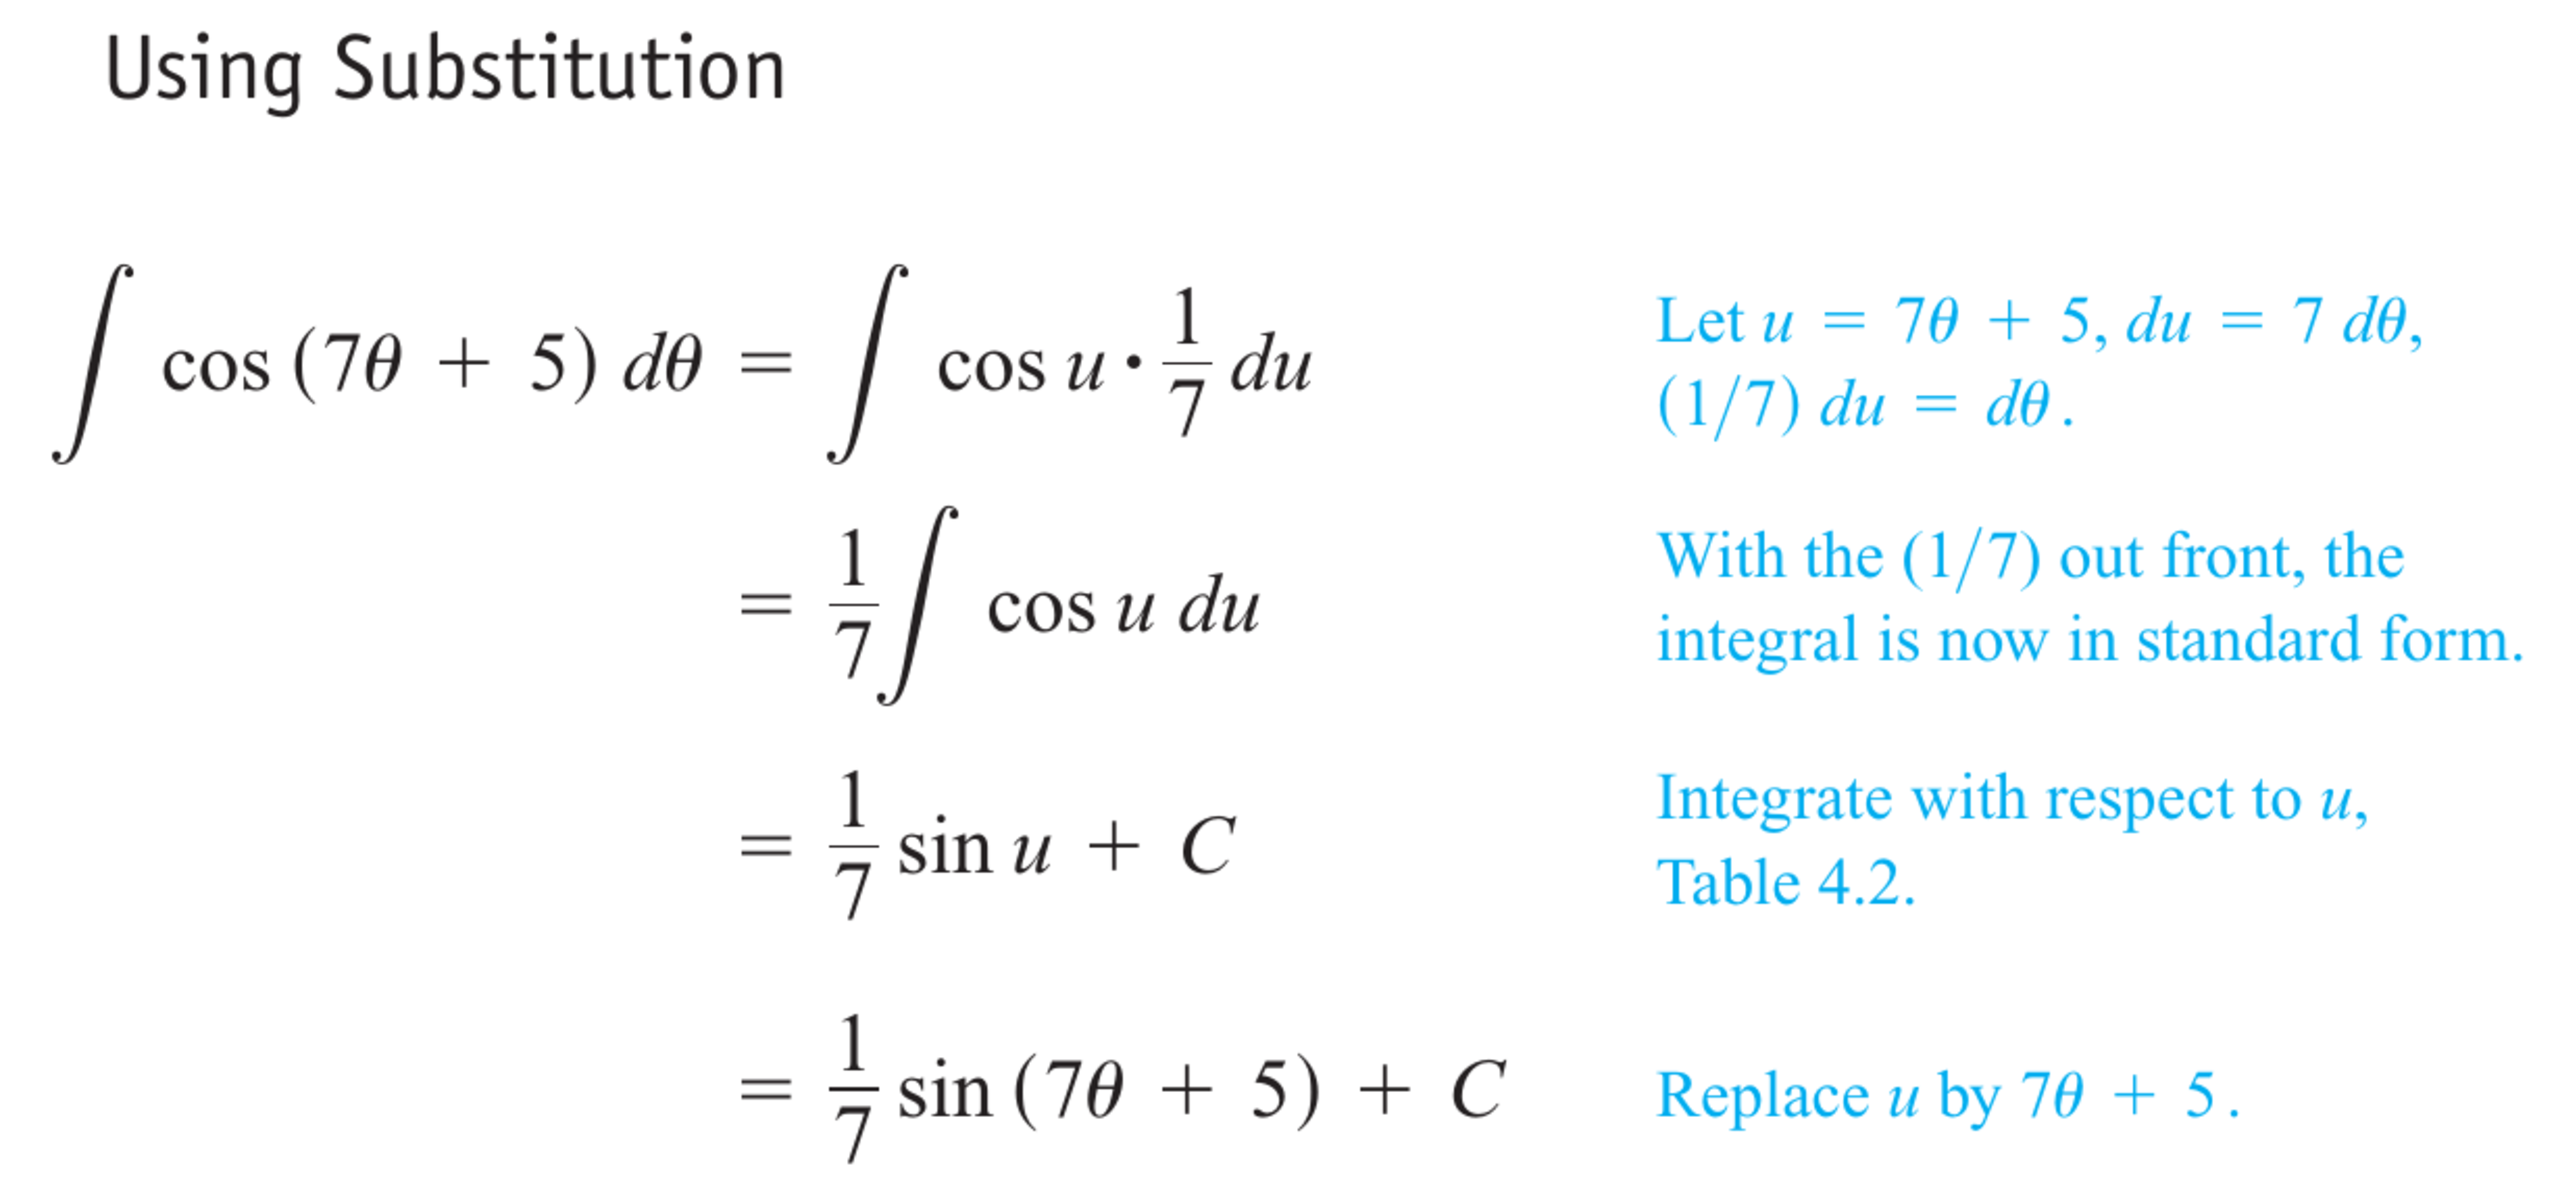
\includegraphics[width=9cm]{2021-2-C2/thomas11-p370-example-3.pdf}$$


Eu comecei a aprender um desses ``programas que entendem
demonstrações'' nas férias -- o Lean:

\ssk

{\footnotesize

\url{https://www.ma.imperial.ac.uk/~buzzard/xena/}

}

\ssk

Ele é considerado muito mais fácil de usar que os ``proof assistants''
anteriores a ele mas ele ainda é bem difícil. Existem tutoriais pra
ele nos quais os usuários têm que demonstrar na linguagem do Lean
montes de exercícios de Matemática Discreta e Cálculo 1, mas acho que
ainda falta bastante pra alunos de primeiro período conseguirem
resolver os seus exercícios na linguagem do Lean.

}\anothercol{

Eu vou fazer algumas referências ao Lean no curso, meio como
curiosidade e meio por conta de uma coisa cuja explicação é meio
longa. Lá vai.

\bsk

Uma das coisas que me dá mais ódio é ter que lidar com alunos que
escrevem um monte de contas totalmente sem pé nem cabeça nas provas e
depois juram que ``tava tudo certo, caramba'' e que eu só dei nota
baixa pra eles porque eu tava de marcação com eles. E tem uma coisa
que me dá tipo 1/100 desse ódio, que é lidar com alunos que fazem
demonstrações nos quais eles pulam montes de passos e juram que tudo
que eles fizeram ``é óbvio''.

Neste curso nós vamos ver as definições \ColorRed{precisas} de {\sl
  alguns tipos} de ``passos óbvios'' que aparecem em demonstrações e
contas que são comuns de Cálculo 2. A maioria das demonstrações que
nós vamos ver são por sequências de igualdades, e vão ter este
formato:

$$\begin{array}{rcll}
    \Expr &=& \Expr & \Just \\
          &=& \Expr & \Just \\
          &=& \Expr & \Just \\
          &=& \Expr & \Just \\
  \end{array}
$$

A operação de substituição que eu vou explicar nos próximos slides vai
servir pra \ColorRed{ZILHÕES} de coisas durante o curso -- entre elas
pra gente entender quais passos da forma abaixo são ``óbvios'':
%
$$\begin{array}{rcll}
    \Expr &=& \Expr & \Just \\
  \end{array}
$$

}}

% (find-thomas11-1page (+ 58 344) "Notation and existence of the definite integral")
% (find-thomas11-1page (+ 61 370) "Example 2")
% (find-thomas11-1page (+ 61 371) "Example 3")

% https://en.wikipedia.org/wiki/Lambda_calculus#Substitution


\newpage

%  ____        _         _   _ _         _                 
% / ___| _   _| |__  ___| |_(_) |_ _   _(_) ___ __ _  ___  
% \___ \| | | | '_ \/ __| __| | __| | | | |/ __/ _` |/ _ \ 
%  ___) | |_| | |_) \__ \ |_| | |_| |_| | | (_| (_| | (_) |
% |____/ \__,_|_.__/|___/\__|_|\__|\__,_|_|\___\__,_|\___/ 
%                                                          
% «substituicao»  (to ".substituicao")
% (c2m212introp 8 "substituicao")
% (c2m212introa   "substituicao")

{\bf Substituição: introdução}

\scalebox{0.4}{\def\colwidth{14cm}\firstcol{

Você deve ter alguma prática de substituições de variáveis ``em
português''... por exemplo,

% (c2m211substp 3 "subst-box")
% (c2m211substa   "subst-box")

\begin{center}
\fbox{\begin{minipage}{7cm}
Se substituirmos $x$ por $10a+b$

e $y$ por $3c+4d$ em:
%
$$x^y + 2x$$
%
obtemos:
%
$$(10a+b)^{3c+4d} + 2(10a+b)$$
\end{minipage}}
\end{center}

E você também deve ter saber substituir funções ``usando português'':

\begin{center}
\fbox{\begin{minipage}{7cm}
Digamos que $f(x)=x^2$. Então:
%
$$\begin{array}{rclcrcl}
  f(200)  &=& 200^2            \\
  f(3u+4) &=& (3u+4)^2         \\
  f(42x^3+99) &=& (42x^3+99)^2 \\[5pt]
  f'(x) &=& 2x \\                
  f'(200) &=& 2·200 \\                
  f'(3u+4) &=& 2(3u+4) \\        
  f'(42x^3+99) &=& 2(42x^3+99) \\
  \end{array}
$$
\end{minipage}}
\end{center}

Como o que você aprendeu em Prog 1 você provavelmente sabe fazer uma
função que recebe um string qualquer e substitui todas as letras
\qco{a} no string por \qqco{oo}s; se essa função receber o string
\qqco{banana} ela retorna \qqco{boonoonoo}. A gente diz que uma função
dessas é ``puramente sintática'' porque ela não se importa com o {\sl
  significado} dos strings \qqco{banana} ou \qqco{boonoonoo}.

}\anothercol{

A nossa operação `$[:=]$' vai servir pra substituir tanto variáveis
quanto funções em expressões matemáticas. No caso mais básico a
sintaxe dela é esta aqui:
%
\def\Expro{\asf{expressão original}}
\def\Exprn{\asf{expressão nova}}
\def\Subst{\asf{substituição}}
\def\Var  {\asf{var}}
\def\Expr {\asf{expr}}
%
$$\begin{array}{rcl}
  \Expro \Subst &=& \Exprn \\[2.5pt]
  \Expro [\Var := \Expr] &=& \Exprn \\
  \end{array}
$$

Ela vai agir da forma mais sintática possível. Essa regra aqui vai ser
\ColorRed{MUITO IMPORTANTE}:

\begin{center}
\fbox{\begin{minipage}{7cm}

    O `$=$' depois de uma substituição tem um significado especial
    (...) a pronúncia dele é ``o resultado da substituição à esquerda
    é a expressão à direita''.

\end{minipage}}
\end{center}

Eu não estou definindo {\sl precisamente} o que isso quer dizer, mas
olhe estes exemplos:
%
$$\begin{array}{rcl}
  (2 = 3 + a·4) \, [a:=5]   &=& (2 = 3 + 5·4) \\
  (2 = 3 + a·4) \, [a:=5+6] &=& (2 = 3 + (5+6)·4) \\
  (2 = 3 + a·4) \, [a:=10]  &=& (2 = 3 + 40) \\
  \end{array}
$$

As duas primeiras linhas seguem a idéia de que ``o resultado da
substituição à esquerda é a expressão à direita'' mas a terceira linha
não -- na terceira a gente tranformou o $10·4$ em 40, e nisso a gente
fez algo a mais além de simplesmente substituir o `$a$' por `10'. 

Aqui as duas primeiras linhas são verdadeiras mas a terceira não,
%
$$\begin{array}{rcl}
          (x^x) \, [x:=2+3] &=& (2+3)^{(2+3)} \\
          (x^x) \, [x:=2+3] &=& (2+3)^{2+3} \\
          (x^x) \, [x:=2+3] &=& 2+3^{2+3} \\
          (x^x) \, [x:=2+3] &=& x^{2+3} \\
  \end{array}
$$
%
porque na terceira a gente omitiu parênteses de um jeito que muda o
significado da expressão original. A quarta linha também é falsa,
porque ``$[x:=2+3]$'' quer dizer ``substitua \ColorRed{TODAS} as
ocorrências da variável $x$ por $2+3$ ou $(2+3)$'', e teve um `$x$'
que a gente não substituiu.

}}



% (c2m211substp 9 "igual-depois-de-subst")
% (c2m211substa   "igual-depois-de-subst")

\newpage

%  ____        _         _   _ _         _                   ____  
% / ___| _   _| |__  ___| |_(_) |_ _   _(_) ___ __ _  ___   |___ \ 
% \___ \| | | | '_ \/ __| __| | __| | | | |/ __/ _` |/ _ \    __) |
%  ___) | |_| | |_) \__ \ |_| | |_| |_| | | (_| (_| | (_) |  / __/ 
% |____/ \__,_|_.__/|___/\__|_|\__|\__,_|_|\___\__,_|\___/  |_____|
%                                                                  
% «substituicao-2»  (to ".substituicao-2")
% (c2m212introp 9 "substituicao-2")
% (c2m212introa   "substituicao-2")


{\bf Substituição: introdução (2)}

\scalebox{0.45}{\def\colwidth{12cm}\firstcol{

A nossa operação `$[:=]$' também vai servir pra substuir funções.
Lembre que:

\begin{center}
\fbox{\begin{minipage}{7cm}
Digamos que $f(x)=x^2$. Então:
%
$$\begin{array}{rclcrcl}
  f(200)  &=& 200^2            \\
  f(3u+4) &=& (3u+4)^2         \\
  f(42x^3+99) &=& (42x^3+99)^2 \\[5pt]
  f'(x) &=& 2x \\                
  f'(200) &=& 2·200 \\                
  f'(3u+4) &=& 2(3u+4) \\        
  f'(42x^3+99) &=& 2(42x^3+99) \\
  \end{array}
$$
\end{minipage}}
\end{center}

Isto aqui vai ser verdade:
%
$$\D \left( \frac{f(200)+5}{f(3u+4)} \right)
  \, \left[ f(x) := x^2 \right]
  \;\; = \;\;
  \left( \frac{200^2+5}{(3u+4)^2} \right)
$$

Agora eu vou introduzir uma gambiarra. A motivação pra ela é a
seguinte: se $f(x) = x^2 \sen x$ então temos dois jeitos equivalentes
de escrever $f'(x)$:
%
$$\begin{array}{rcl}
  f'(x) &=& 2x·\sen x + x^2 \cos x \\
  f'(x) &=& x^2 \cos x + 2x·\sen x \\
  \end{array}
$$

Se a gente não decide de antemão qual das duas expressões pra $f'(x)$
a gente vai usar fica muito mais difícil -- pelo menos pra mim, que
sou péssimo em contas -- calcular o resultado de uma substituição como
esta:
%
$$\D \left( \frac{42+f(x)}{f'(x)} \right)
  \, \left[ f(x) := x^2 \sen x \right]
  \;\; = \;\;
  \ColorRed{?}
$$

}\anothercol{

A gambiarra é que em substituições como a acima, em que tanto $f(x)$
quanto $f'(x)$ vão ter que ser substituídos, a gente sempre vai
escrever linhas novas na caixinha das substituições pra ajudar, e
essas linhas novas vão ser \ColorRed{consequências das linhas de
  cima}. Por exemplo, a substituição acima pode virar isto,
%
$$\D \left( \frac{42+f(x)}{f'(x)} \right)
  \, \bmat{ f(x) := x^2 \sen x \\ f'(x) := 2x·\sen x + x^2 \cos x }
  \;\; = \;\;
  \ColorRed{?}
$$
%
mas também poderíamos ter usado o $f'(x)$ na outra ordem.

\bsk

Uma das vantagens do `$[:=]$' ser uma operação ``puramente sintática''
é que podemos aplicar o `$[:=]$' a expressões cujo significado a gente
ainda não entende. Nós vamos usar isto muitas vezes no curso pra
entender definições que parecem complicadas porque são muito gerais. O
`$[:=]$' nos permite obter casos particulares que são fáceis de
entender.


\bsk
\bsk
\bsk

\ColorRed{\bf Exercício 1.}

Quando eu corrigi as P1s do semestre passado eu vi que muitas pessoas
ainda tinham muita dificuldade com o `$[:=]$', e aí depois de fazer o
gabarito dela eu pus um apêndice no PDF da P1 com exercícios baseados
no gabarito. Tente fazer o exercício da página 17; a definição da
fórmula $[\textsf{S2I}]$ está na página 7. Link:

\ssk

{\footnotesize

% (c2m211p1p 14 "apendice")
% (c2m211p1a    "apendice")
%    http://angg.twu.net/LATEX/2021-1-C2-P1.pdf#page=14
\url{http://angg.twu.net/LATEX/2021-1-C2-P1.pdf\#page=14}

}

}}





\newpage

%  _____                   _      _         _ 
% | ____|_  _____ _ __ ___(_) ___(_) ___   / |
% |  _| \ \/ / _ \ '__/ __| |/ __| |/ _ \  | |
% | |___ >  <  __/ | | (__| | (__| | (_) | | |
% |_____/_/\_\___|_|  \___|_|\___|_|\___/  |_|
%                                             
% «exercicio-1»  (to ".exercicio-1")
% (c2m212introp 10 "exercicio-1")
% (c2m212introa    "exercicio-1")

{\bf Exercício 1.}

\def\StwoIsetargs #1{\StwoIsetargss #1}
\def\StwoIsetargss#1#2#3#4#5#6{
  \sa{x}{#1} \sa{u}{#2} \sa{gx}{#3} \sa{g'x}{#4}
  \sa{nw}{F(\ga{gx})}   \sa{ne}{#5}
  \sa{sw}{F(\ga{u})}    \sa{se}{#6}
  }
\def\StwoItmp{
  \isubstboxTT
    {\ga{nw}}  {\int \ga{ne} \, d\ga{x}}
    {\ph{m}}
    {\ga{sw}}  {\int \ga{se} \, d\ga{u}}
    {Se $F'(\ga{u})=\ga{se}$ então:}
    {Obs:  $\ga{u} =\ga{gx}$.}
}
\def\StwoIsubsts{
  \bmat{x:=\ga{x} \\
        u:=\ga{u} \\
        f(\ga{u}):=\ga{se} \\
        g(\ga{x}):=\ga{gx} \\
       g'(\ga{x}):=\ga{g'x} \\
       }
}

\scalebox{0.55}{\def\colwidth{10cm}\firstcol{

    Este é o ``Exercício 1'' do apêndice do gabarito da P1 do semestre
    passado, ligeiramente rearrumado e incluindo as dicas.

    No semestre passado nós definimos a \pfo{S2I} -- que é uma
    demonstração! -- deste jeito:
    %
    $$ \pfo{S2I} \;\;=\;\; \StwoI $$

    Nós vamos usar ``\pfo{S2I}'' como uma {\sl abreviação} pra essa
    coisa grandona entre parênteses.

    Copie a \pfo{S2I} -- a versão ``por extenso'' dela, à direita do
    `$=$' -- pra uma folha de papel e \ColorRed{recorte isso} pra você
      poder reusar essa \pfo{S2I} ``por extenso'' sem precisar
      copiá-la várias vezes. É sério, esse tuque da \pfo{S2I}
    recortada vai te poupar muito tempo! Depois encontre os resultados
    das quatro substituições da coluna da direita e compare-os com o
    gabarito do próximo slide.



}\anothercol{

\def\eqq{\;\; = \;\; \Rd{?}}

$$\scalebox{1.0}{$
  \begin{array}{l}
    \StwoIsetargs{ {x} {u} {3x} {3}
                    {\frac{\cos(2+\sqrt{3x+4})}{2\sqrt{3x+4}}·3}
                    {\frac{\cos(2+\sqrt{ u+4})}{2\sqrt{ u+4}}  } }
    a) \;\; \pfo{S2I} \StwoIsubsts \eqq
    %
    \\[40pt]
    %
    \StwoIsetargs{ {u} {v} {u+4} {1}
                    {\frac{\cos(2+\sqrt{u+4})}{2\sqrt{u+4}}·1}
                    {\frac{\cos(2+\sqrt{ v })}{2\sqrt{ v }}} }
    b) \;\; \pfo{S2I} \StwoIsubsts \eqq
    %
    \\[40pt]
    %
    \StwoIsetargs{ {v} {w} {\sqrt{v}} {(2\sqrt{v})^{-1}}
                    {\cos(2+\sqrt{v}) ·(2\sqrt{v})^{-1}}
                    {\cos(2+w)} }
    c) \;\; \pfo{S2I} \StwoIsubsts \eqq
    %
    \\[40pt]
    %
    \StwoIsetargs{ {w} {y} {2+w} {1}
                    {\cos(2+w)·1}
                    {\cos(y)} }
    d) \;\; \pfo{S2I} \StwoIsubsts \eqq
    \\
  \end{array}
  $}
$$

}}

\newpage

%  _____                   _      _         _               _     
% | ____|_  _____ _ __ ___(_) ___(_) ___   / |   __ _  __ _| |__  
% |  _| \ \/ / _ \ '__/ __| |/ __| |/ _ \  | |  / _` |/ _` | '_ \ 
% | |___ >  <  __/ | | (__| | (__| | (_) | | | | (_| | (_| | |_) |
% |_____/_/\_\___|_|  \___|_|\___|_|\___/  |_|  \__, |\__,_|_.__/ 
%                                               |___/             
% «exercicio-1-gab»  (to ".exercicio-1-gab")
% (c2m212introp 11 "exercicio-1-gab")
% (c2m212introa    "exercicio-1-gab")

{\bf Gabarito do Exercício 1}

\ssk

$\scalebox{0.45}{$
  \begin{array}{l}
    \StwoIsetargs{ {x} {u} {3x} {3}
                    {\frac{\cos(2+\sqrt{3x+4})}{2\sqrt{3x+4}}·3}
                    {\frac{\cos(2+\sqrt{ u+4})}{2\sqrt{ u+4}}  } }
    \StwoI \StwoIsubsts \;\;=\;\; \StwoItmp
    %
    \\[55pt]
    %
    \StwoIsetargs{ {u} {v} {u+4} {1}
                    {\frac{\cos(2+\sqrt{u+4})}{2\sqrt{u+4}}·1}
                    {\frac{\cos(2+\sqrt{ v })}{2\sqrt{ v }}} }
    \StwoI \StwoIsubsts \;\;=\;\; \StwoItmp
    %
    \\[55pt]
    %
    \StwoIsetargs{ {v} {w} {\sqrt{v}} {(2\sqrt{v})^{-1}}
                    {\cos(2+\sqrt{v}) ·(2\sqrt{v})^{-1}}
                    {\cos(2+w)} }
    \StwoI \StwoIsubsts \;\;=\;\; \StwoItmp
    %
    \\[55pt]
    %
    \StwoIsetargs{ {w} {y} {2+w} {1}
                    {\cos(2+w)·1}
                    {\cos(y)} }
    \StwoI \StwoIsubsts \;\;=\;\; \StwoItmp
    \\
  \end{array}
  $}
$



\newpage

%  _____ ____   ___             _           _             
% | ____|  _ \ / _ \ ___    ___| |__  _   _| |_ __ _ _ __ 
% |  _| | | | | | | / __|  / __| '_ \| | | | __/ _` | '__|
% | |___| |_| | |_| \__ \ | (__| | | | |_| | || (_| | |   
% |_____|____/ \___/|___/  \___|_| |_|\__,_|\__\__,_|_|   
%                                                         
% «EDOs-chutar-testar»  (to ".EDOs-chutar-testar")
% (c2m212introp 12 "EDOs-chutar-testar")
% (c2m212introa    "EDOs-chutar-testar")

{\bf EDOs por chutar e testar}


\scalebox{0.45}{\def\colwidth{12.5cm}\firstcol{

Eu costumava começar o curso por este exercício aqui:

\ssk

{\footnotesize

% (c2m202introp 4 "EDOs")
% (c2m202introa   "EDOs")
%    http://angg.twu.net/LATEX/2020-2-C2-intro.pdf#page=4
\url{http://angg.twu.net/LATEX/2020-2-C2-intro.pdf\#page=4}

}

\msk

Considere estas equações:
%
$$
\begin{array}{rll}
 1) & x+2   = 5              \\
 2) & x^2+3 = 7              \\
 3) & x^2+x = 6              \\[5pt]
 4) & f'(x) = x^4            \\
 5) & f'(x) = 2f(x)          \\
 6) & f''(x) + f'(x) = 6f(x) \\
 7) & f'(x) = -1/f(x)        \\
 8) & f'(x) = -x/f(x)        \\
 \end{array}
$$

As equações 1--3 são equações ``comuns'' em que temos que encontrar
valores de $x$ que satisfaçam a igualdade e as equação 4--8 são EDOs
em que temos que encontrar \ColorRed{funções} $f$ que satisfaçam a
igualdade \ColorRed{para todo $x$ no domínio de $f$}. A sugestão pros
exercícios 4--8 é: \ColorRed{comece} testando as `$f$'s abaixo...
%
$$\begin{array}{rll}
  f(x) &=& x^3,           \\
  f(x) &=& x^5,           \\
  f(x) &=& 200x^5 + 42,   \\
  f(x) &=& e^x,           \\
  f(x) &=& e^{42x},       \\
  f(x) &=& e^{2x},        \\
  f(x) &=& e^{3x},        \\
  f(x) &=& \sqrt{1-x^2},  \\
  f(x) &=& \sqrt{4-x^2}.  \\
  \end{array}
$$


}\anothercol{

  Normalmente esses testes são feitos usando Português. Por exemplo:

  \begin{quote}
    Vamos tentar encontrar soluções para a EDO $f'(x) = x^4$ por
    chutar-e-testar. Vamos ver se $f(x) = x^3$ é uma solução para esta
    EDO. Substituindo $f(x)$ por $f(x) = x^3$ na EDO $f'(x) = x^4$
    obtemos $3x^2 = x^4$; esta igualdade não é verdadeira para todo
    $x$, então a função $f(x) = x^3$ não é uma solução para a EDO
    $f'(x) = x^4$.
  \end{quote}

  A parte em que todo mundo se enrola é o ``Substituindo $f(x)$ por
  $f(x) = x^3$ na EDO $f'(x) = x^4$ obtemos...''. Como o `$[:=]$' nós
  podemos escrever esse passo como:
  %
  $$(f'(x) = x^4) \; \Subst{f(x) := x^3 \\ f'(x) := 3x^2}
    \;\; = \;\; (3x^2 = x^4)
  $$
  %
  e temos
  %
  $$(∀x∈\R.\; 3x^2 = x^4) \;\;=\;\; \False.$$

  O domínio da função $f(x) = x^3$ é $\R$, e por isso eu usei
  ``$∀x∈\R$'' logo acima. Em Cálculo 2 muitos detalhes, como os
  domínios das funções, ou só são preenchidos no final ou são deixados
  implícitos (``a cargo do leitor'')... aí os livros normalmente vão
  dizer só algo como ``$3x^2 = x^4$ é falso'' e você vai ter que
  descobrir os detalhes por si mesmo.

  \bsk

  {\bf \ColorRed{Exercício 2.}}

  Encontre soluções das EDOs 4--8 por chutar-e-testar. Use as `$f$'s
  sugeridas à esquerda.

}}


\newpage

%  ____                        _             _           
% / ___|  ___  _ __ ___   __ _| |_ ___  _ __(_) ___  ___ 
% \___ \ / _ \| '_ ` _ \ / _` | __/ _ \| '__| |/ _ \/ __|
%  ___) | (_) | | | | | | (_| | || (_) | |  | | (_) \__ \
% |____/ \___/|_| |_| |_|\__,_|\__\___/|_|  |_|\___/|___/
%                                                        
% «somatorios»  (to ".somatorios")
% (c2m212introp 13 "somatorios")
% (c2m212introa    "somatorios")


{\bf Somatórios}


\scalebox{0.45}{\def\colwidth{12cm}\firstcol{

    O material desta página foi adaptado daqui:

    \ssk

    {\footnotesize

      % (c2m211substp 19 "somatorios")
      % (c2m211substa    "somatorios")
      % http://angg.twu.net/LATEX/2021-1-C2-subst.pdf#page=19
      \url{http://angg.twu.net/LATEX/2021-1-C2-subst.pdf\#page=19}

    }

    \bsk

    Antigamente somatórios eram matéria de ensino médio, mas hoje em
    dia muita gente chega em Cálculo 2 sem nunca ter visto
    somatórios...

    As fórmulas para somas de progressões aritméticas (PAs) e para
    somas de progressões geométricas (PGs) usam `$\sum$'s. Veja:

    \bsk

    {\footnotesize

      % https://pt.wikipedia.org/wiki/Progress%C3%A3o_aritm%C3%A9tica
      \url{https://pt.wikipedia.org/wiki/Progress\%C3\%A3o_aritm\%C3\%A9tica}

      % https://pt.wikipedia.org/wiki/Progress%C3%A3o_geom%C3%A9trica
      \url{https://pt.wikipedia.org/wiki/Progress\%C3\%A3o_geom\%C3\%A9trica}

      % https://pt.wikipedia.org/wiki/Somat%C3%B3rio
      \url{https://pt.wikipedia.org/wiki/Somat\%C3\%B3rio}

    }

    % «soma-PG»  (to ".soma-PG")
    % (c2m212introp 13 "soma-PG")
    % (c2m212introa    "soma-PG")
    % (c2m211substp 13 "soma-PG")
    % (c2m211substa    "soma-PG")

    \bsk

    Relembre:
    % 
    $$\scalebox{0.9}{$
      \begin{array}{rcl}
        \sum_{k=2}^{5} 10^k &=& 10^2 + 10^3 + 10^4 + 10^5 \\
                            &=& 100 + 1000 + 10000 + 100000 \\
                            &=& 111100 \\
        (1-10) \sum_{k=2}^{5} 10^k &=& (1-10)(100 + 1000 + 10000 + 100000) \\
                            &=& (100 + 1000 + 10000 + 100000) \\
                            && - (1000 + 10000 + 100000 + 1000000) \\
                            &=& 100 - 1000000 \\
                            &=& 10^2 - 10^{5+1} \\
        \sum_{k=2}^{5} 10^k &=& \D \frac{10^2 - 10^{5+1}}{1-10} \\
      \end{array}
      $}
    $$

    A fórmula geral é: \quad
    % 
    $\D \sum_{k=a}^{b} x^k
    \; = \;
    \D \frac{x^a - x^{b+1}}{1 - x}
    \; = \;
    \D \frac{x^{b+1}- x^a}{x - 1}
    $
    \;.

}\anothercol{

  % «somatorio-expansao»  (to ".somatorio-expansao")
  % (c2m212introp 13 "somatorio-expansao")
  % (c2m212introa    "somatorio-expansao")

  Repare que dá pra calcular o somatório do início do slide anterior
  em mais passos usando o `$[:=]$'...

  $$\scalebox{0.9}{$
    \begin{array}{rcl}
      \sum_{k=2}^{5} 10^k &=& 10^2 + 10^3 + 10^4 + 10^5 \\[5pt]
      \sum_{k=2}^{5} 10^k &=& (10^k) [k:=2] \\
                          &+& (10^k) [k:=3] \\
                          &+& (10^k) [k:=4] \\
                          &+& (10^k) [k:=5] \\[2.5pt]
                          &=& 10^2 + 10^3 + 10^4 + 10^5 \\
    \end{array}
    $}
  $$
  
  Às vezes a gente vai usar esse passo intermediário com `$[:=]$'s pra
  não se enrolar em somatórios de expressões complicadas... Por
  exemplo aqui, e nas páginas seguintes:

  \ssk

  % (c2m211somas1p 12 "partition-sum")
  % (c2m211somas1a    "partition-sum")
  % http://angg.twu.net/LATEX/2021-1-C2-somas-1.pdf#page=12
  {\footnotesize
    
    \url{http://angg.twu.net/LATEX/2021-1-C2-somas-1.pdf\#page=12}
    
  }

  \bsk

  % «somatorios-exercs»  (to ".somatorios-exercs")
  % (c2m212introp 13 "somatorios-exercs")
  % (c2m212introa    "somatorios-exercs")
  % (c2m211substp 22 "somatorios-exercs")
  % (c2m211substa    "somatorios-exercs")
  
  {\bf \ColorRed{Exercício 3:}}
  
  \ssk
  
  Expanda e calcule:
  
  a) $\sum_{n=1}^5 (2n-1)$
  
  \ssk
  
  b) $\sum_{n=0}^4 (2n+1)$
  
  \msk
  
  c) $\sum_{k=0}^2 (k+1)$
  
  \msk
  
  d) $\sum_{k=0}^2 k + 1$
  
  \msk
  
  e) $\left( \sum_{k=0}^2 k \right) +1$
  
  \msk
  
  Expanda e calcule/simplifique até onde der:
  
  f) $\sum_{n=1}^5 (2k-1)$
  
  \ssk
  
  g) $\sum_{k=1}^5 (2n-1)$
  
  \ssk
  
  h) $\sum_{n=4}^6 f(10n)$
  
  \ssk

  i) $\sum_{n=4}^6 f(10n)$, onde $f(x) = 10x$

}}






% (c2m211p1p 14 "apendice")
% (c2m211p1a    "apendice")
% (c2m211p1p 17 "exercicio")
% (c2m211p1a    "exercicio")
% (c2m211substp 28 "depoimento-pessoal")
% (c2m211substa    "depoimento-pessoal")
%    http://angg.twu.net/LATEX/2021-1-C2-subst.pdf#page=28
%\url{http://angg.twu.net/LATEX/2021-1-C2-subst.pdf\#page=28}



% (c2m211substp 9 "dicas-subst")
% (c2m211substa   "dicas-subst")




% Tipos de =




%\printbibliography

\GenericWarning{Success:}{Success!!!}  % Used by `M-x cv'

\end{document}

%  ____  _             _         
% |  _ \(_)_   ___   _(_)_______ 
% | | | | \ \ / / | | | |_  / _ \
% | |_| | |\ V /| |_| | |/ /  __/
% |____// | \_/  \__,_|_/___\___|
%     |__/                       
%
% «djvuize»  (to ".djvuize")
% (find-LATEXgrep "grep --color -nH --null -e djvuize 2020-1*.tex")

 (eepitch-shell)
 (eepitch-kill)
 (eepitch-shell)
# (find-fline "~/2021.2-C2/")
# (find-fline "~/LATEX/2021-2-C2/")
# (find-fline "~/bin/djvuize")

cd /tmp/
for i in *.jpg; do echo f $(basename $i .jpg); done

f () { rm -v $1.pdf;  textcleaner -f 50 -o  5 $1.jpg $1.png; djvuize $1.pdf; xpdf $1.pdf }
f () { rm -v $1.pdf;  textcleaner -f 50 -o 10 $1.jpg $1.png; djvuize $1.pdf; xpdf $1.pdf }
f () { rm -v $1.pdf;  textcleaner -f 50 -o 20 $1.jpg $1.png; djvuize $1.pdf; xpdf $1.pdf }

f () { rm -fv $1.png $1.pdf; djvuize $1.pdf }
f () { rm -fv $1.png $1.pdf; djvuize WHITEBOARDOPTS="-m 1.0 -f 15" $1.pdf; xpdf $1.pdf }
f () { rm -fv $1.png $1.pdf; djvuize WHITEBOARDOPTS="-m 1.0 -f 30" $1.pdf; xpdf $1.pdf }
f () { rm -fv $1.png $1.pdf; djvuize WHITEBOARDOPTS="-m 1.0 -f 45" $1.pdf; xpdf $1.pdf }
f () { rm -fv $1.png $1.pdf; djvuize WHITEBOARDOPTS="-m 0.5" $1.pdf; xpdf $1.pdf }
f () { rm -fv $1.png $1.pdf; djvuize WHITEBOARDOPTS="-m 0.25" $1.pdf; xpdf $1.pdf }
f () { cp -fv $1.png $1.pdf       ~/2021.2-C2/
       cp -fv        $1.pdf ~/LATEX/2021-2-C2/
       cat <<%%%
% (find-latexscan-links "C2" "$1")
%%%
}

f thomas11-p370-example-3

f 20201213_area_em_funcao_de_theta
f 20201213_area_em_funcao_de_x
f 20201213_area_fatias_pizza



%  __  __       _        
% |  \/  | __ _| | _____ 
% | |\/| |/ _` | |/ / _ \
% | |  | | (_| |   <  __/
% |_|  |_|\__,_|_|\_\___|
%                        
% <make>

 (eepitch-shell)
 (eepitch-kill)
 (eepitch-shell)
# (find-LATEXfile "2019planar-has-1.mk")
make -f 2019.mk STEM=2021-2-C2-intro veryclean
make -f 2019.mk STEM=2021-2-C2-intro pdf

% «elisp»  (to ".elisp")

(defun cols () (interactive) (insert "
\\scalebox{0.6}{\\def\\colwidth{9cm}\\firstcol{
}\\anothercol{
}}
"))

% Local Variables:
% coding: utf-8-unix
% ee-tla: "c2i"
% ee-tla: "c2m212intro"
% End:
